%! Author = drakanoy
%! Date = 10.09.2024

% Preamble
\documentclass[12pt]{article}

% Packages
\usepackage[utf8]{inputenc}
\usepackage[T2A]{fontenc}
\usepackage[english, russian]{babel}
\usepackage[a4paper, includefoot, left=1.5cm, right=1.5cm, top=1cm, bottom=1.5cm, headsep=1cm, footskip=1cm]{geometry}
\usepackage{makecell}
\usepackage{amsmath}
\usepackage{graphicx}
\usepackage{enumitem}
\usepackage{svg}
\usepackage{multirow}
\usepackage{hyperref}
\usepackage{mathtools}

% Document
\begin{document}
\begin{large}
\begin{center}
\LARGE \textbf{Домашняя работа}
\par
\LARGE \textbf{Кононов Александр Михайлович}
\par
    \textbf{10.09.2024}
\end{center}
\par Условие:
\par
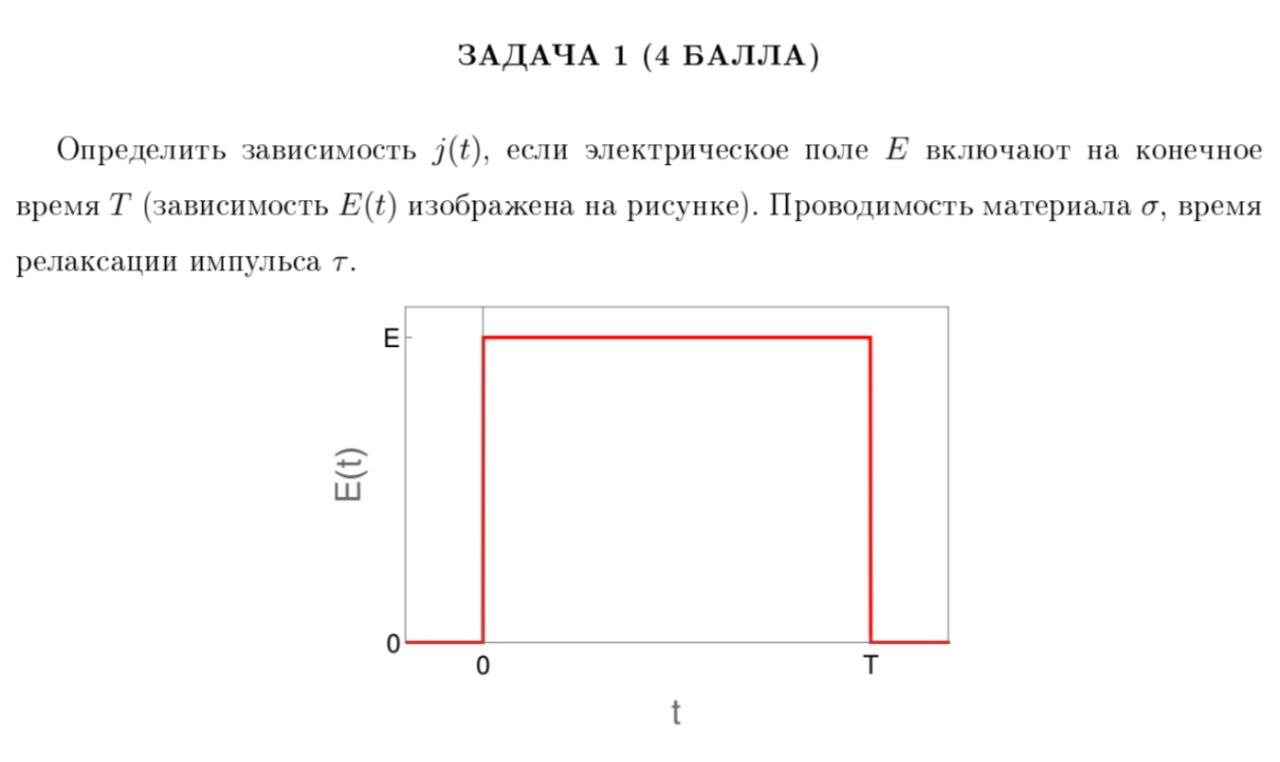
\includegraphics[width=\textwidth]{photo.jpg}
%\begin{center}
%\underline{Рисунок 1}:
%\end{center}
\par Решение:
\[
    j(t) = \frac{\sigma}{\tau} \int\limits_0^{+\infty} E(t-\widetilde{t} ) e^{-\widetilde{t}/\tau} d \widetilde{t}
\]
\[
    E(t) =
    \begin{cases}
        0; t < 0
        \\
        E; 0 < t < T
        \\
        0; t > T
    \end{cases}
\]
\par Сделаем замену в интеграле:
\[
    t - \widetilde{t} = y
\]
\[
    - \widetilde{t} = y - t
\]
\[
    d \widetilde{t} = -dy
\]
\[
    \widetilde{t} = 0 <=> y = t
\]
\[
    \widetilde{t} = + \infty <=> y = - \infty
\]
\par Тогда
\[
    j(t) = \frac{\sigma}{\tau} \int\limits_0^{+\infty} E(t-\widetilde{t} ) e^{-\widetilde{t}/\tau} d \widetilde{t} =
\]
\[
    = \frac{\sigma}{\tau} \int\limits_{-\infty}^{t} E(y) e^{(y-t)/\tau} dy = \frac{\sigma}{\tau} e^{-t/\tau} E \int\limits_{0}^{t} e^{y/\tau}dy =
\]
\[
    = \frac{\sigma}{\tau} E e^{-t/\tau}
    \begin{cases}
        \int\limits_{0}^{T} e^{y/\tau} dy ; t > T
        \\
        \int\limits_{0}^{t} e^{y/\tau} dy ; 0 < t < T
        \\
        0 ; t < 0
    \end{cases}
\]
\[
    = \frac{\sigma}{\tau} E \tau e^{-t/\tau}
    \begin{cases}
        e^{y/\tau}  \textbar_{0}^{T} ; t > T
        \\
        e^{y/\tau}  \textbar_{0}^{t} ; 0 < t < T
        \\
        0 ; t < 0
    \end{cases}
\]
\[
    = \sigma E e^{-t/\tau}
    \begin{cases}
        (e^{T/\tau} - 1) ; t > T
        \\
        (e^{t/\tau} - 1)  ; 0 < t < T
        \\
        0 ; t < 0
    \end{cases}
\]
\[
    = \sigma E e^{-t/\tau} [(e^{T/\tau} - 1) \cdot \Theta(t - T) + (e^{t/\tau} - 1) \cdot (\Theta(t) - \Theta(t - T) )]
\]
\par Ответ:
\[
   j(t) = \sigma E e^{-t/\tau} [(e^{T/\tau} - 1) \cdot \Theta(t - T) + (e^{t/\tau} - 1) \cdot (\Theta(t) - \Theta(t - T) )]
\]
\end{large}
\end{document}
